\chapter{OpenID Based Solution}
In this chapter we will provide a solution using OpenID based IMS. We will give more details about how this system can be implemented, and how it will behave for the end users.
\section{OpenID IMS}
We can replace IMS with \textit{OpenID based IMS} in our pseudonymous system. This system will take the user's credentials and then send the pseudonym, account ID and policy to the bank. This IMS can be controlled by a separate identity inside the bank or by a 3rd party.
\begin{figure}[h]
	\centering
	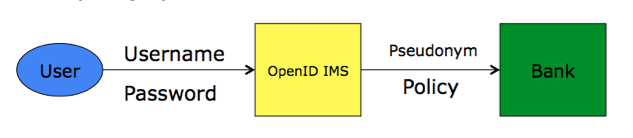
\includegraphics[width=\textwidth]{figures/OpenID}
	\caption{Pseudonym System with OpenID IMS}
	\label{fig:OpenID}
\end{figure}
\section{System Setup}
The system can be setup in two ways:
\begin{itemize}
	\item IMS controlled by a separate department at the bank.
	
	In this case the bank separates the authentication and the service part in two different departments internally. Authentication is controlled by IMS which holds the sensitive user data but the service department doesn't need to have access to that data to provide services to the user.
	\item IMS controlled by a third party.
	
	In this case the bank operates the service part while the authentication part is operated by a trusted third party.
\end{itemize}
In both cases, the bank and the IMS have to collaborate and the bank has to trust the IMS system that the pseudonym and the policy sent by the IMS system are correct.
\subsection{Changes on the Bank Side}
In order to provide services using a pseudonym, the bank needs to have a temporary policy database at its end. So that when the bank gets the pseudonym and the policy from the IMS system, it can store that policy with the pseudonym and provide the services according to the policy.
\subsection{Information Stored at IMS}
IMS needs the following user information to be stored:
\begin{itemize}
	\item User ID
	\item Account ID
	\item Policy
\end{itemize}
The account ID and the policy can be stored in an encrypted form, which can then only be opened by the bank. OpenID IMS also needs to store a \textit{mapping database} from the user ID to the pseudonym for escrow purposes.
\subsection{Changes needed on the User's Side}
On the user's side no changes are needed. The user accesses the system like before. The user doesn't need to install any special software or hardware on his side to access the services of the bank. 
\section{User Creation}
Below are the steps for creation of a new user account in an OpenID based system:
\begin{itemize}
	\item A user goes to the bank to open a new account.
	\item The user provides his details.
	\item The bank creates the user policy and sends this information to the IMS system along with other user information.
	\item The IMS system verifies the user information and provides the user with credentials to access his account.
	\item The user can then login to his account using the credentials.
	\item In case of corporate users, if the user is the administrator then he can add more users by means of a web interface at the IMS system directly and decide the account policies for those users.
\end{itemize}
\section{User Authentication}
Authentication steps are as follows in OpenID based system:
\begin{itemize}
	\item The user goes to login page.
	\item The user provides his username and password.
	\item This is sent to OpenID IMS which verifies the user and creates a pseudonym for the given user ID.
	\item This user ID to the pseudonym mapping is stored in the database for escrow purposes.
	\item The IMS gets the policy for the given user ID from the policy database.
	\item The IMS then sends the pseudonym, account ID and policy to the bank. 
	\item The bank gets this information and creates a temporary policy for the given pseudonym.
	\item The user can then access services from the bank using the pseudonym.
	\item All the user's transactions are logged with the pseudonym.
\end{itemize}
\section{ID Escrow}
Following are the steps for ID escrow in OpenID based system:
\begin{itemize}
	\item The authorities come to the bank for the transaction data.
	\item After verifying, bank gives the transaction data to the authorities.
	\item The authorities then go to the IMS based system for the mapping data.
	\item After verifying, the  IMS gives the mapping data to the authorities.
	\item The authorities then get the real identity of the user from the mapping and transaction data.
\end{itemize}
\section{Analysis}
With the use of OpenID IMS we add a \textit{pseudonymous layer} in the system. This provides us the necessary privacy. But in order to do so, the OpenID provider needs access to a lot of data. Some of the example data is:
\begin{itemize}
	\item UserID
	\item Account ID 
	\item Policies	
\end{itemize}
In addition to that, the provider needs to store the mapping database from the userID to the pseudonym. The bank really has to trust the provider with storage of all this sensitive data. In some cases the bank might not want the provider to store such data on their premises.

In case there is a discrepancy, the authorities need to go both to the bank to get the transaction data, as well as the provider for the mapping data.
\section {OpenID implementation in the Real World}
Now we will try to fit this implementation in our system, which includes Nykredit as the Bank, Signicat as the 3rd party, DTU as the corporate customer and other government institutions as the authorities.
\subsection{Addition of the New User}
Addition of the new user can happen as follows:
\begin{enumerate}
	\item DTU registers the new user with Nykredit giving them the user details and policies that should apply to the particular user regarding the account. 
	\begin{enumerate}
		\item Nykredit registers this new user with his user ID with the IMS system. Nykredit also adds policy for the user in the IMS system.
	\end{enumerate}
	\item Nykredit issues user credentials for the given user to DTU.
	\item DTU then uses this policy credentials to register the new user with Signicat. 
	\begin{enumerate}
		\item Signicat inquires about the user data with the authorities.
		\item The authorities verify the user data to Signicat.
	\end{enumerate}
	\item After that Signicat issues the final OpenID credentials for the IMS system.  These credentials are then used to login to the IMS system by the new user.
\end{enumerate}
\begin{figure}[h]
	\centering
	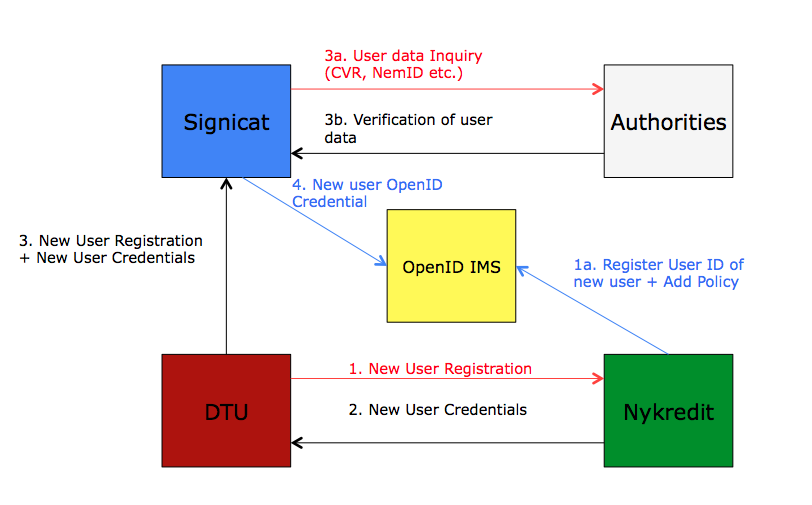
\includegraphics[width=\textwidth]{figures/OpenID-Real}
	\caption{OpenID Registration for a new user}
	\label{fig:OpenID-Real}
\end{figure}

\FloatBarrier
\subsection{Addition of a New Customer}
Addition of a new customer is almost the same as the addition of a new user:
\begin{enumerate}
	\item An administrator goes to Nykredit to open a bank account on behalf of DTU. 
	\begin{enumerate}
		\item Nykredit registers DTU as a new customer in their internal system.
		\item Nykredit register the DTU administrator with his user ID with the IMS system.
	\end{enumerate}
	\item Nykredit issues user credentials for the  DTU administrator.
	\item The administrator then uses these credentials to register himslef as an owner of the new DTU account with Signicat. 
	\begin{enumerate}
		\item Signicat inquires about the data given in the credential with the authorities.
		\item The authorities verify the data to Signicat.
	\end{enumerate}
	\item After that, Signicat issues the final OpenID credentials for the IMS system. These credentials are then used to login to the IMS system by the administrator.
\end{enumerate}
\subsection{Technical Requirements}
In this system, DTU as a client doesn't need to change anything on their side to be a customer at Nykredit. All the system for DTU is web based, where they can just add/remove users. Moreover, DTU users login to the system using the normal web browser.

Nykredit has to implement the OpenID relying party service on their side. In this case they have to store the sensitive data with the 3rd party. The account details and policies are stored at IMS.

Signicat has to implement the OpenID identity provider service on their side.

IMS has to implement the OpenID identity provider service on their side.
The details of the implementation of these services can be found in \cite{recordon2006openid}.

This chapter described the IMS system setup using the OpenID system. We described how the system will be setup and how it will affect all the parties involved. Finally we discussed how OpenID IMS will be implemented in the real world scenario.

